Como enunciamos en la explicaci\'on de nuestro algoritmo, el mismo va chequeando en cada paso si existe alg\'un gimnasio capaz de ser vencido y si existe buscar cual es el m\'as cercano de estos a ser vencidos, por lo tanto existir\'an casos en los cuales la soluci\'on obtenida para los mismos sea la \'optima pero para algunos no lo ser\'a.

Se obtendr\'a la soluci\'on \'optima cuando se reciban pokeparadas y gimnasios en orden, o sea, primero pokeparadas para vencer a un gimnasio cerca de ellas y luego m\'as pokeparadas para vencer a otros gimnasios que se encuentren cerca de estas \'ultimas, se mostrar\'a a continuaci\'on un dibujo que ejemplifica lo dicho:

\vspace*{0.3cm} \vspace*{0.3cm}
  \begin{center}
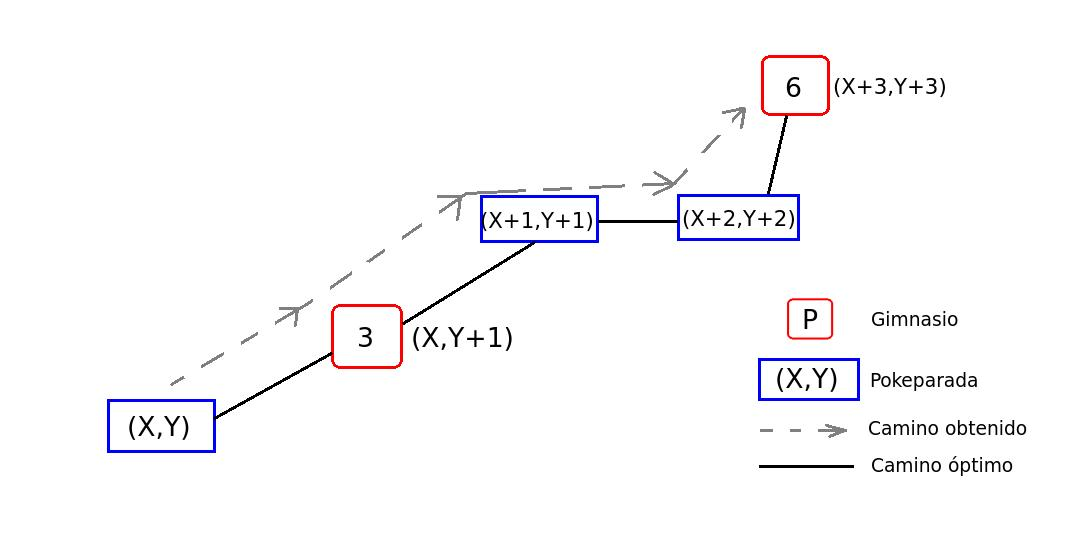
\includegraphics[scale=0.60]{./EJ2/optima.jpeg}
\\{\textit{La soluci\'on obtenida es la \'optima}}
  \end{center}
  \vspace*{0.3cm}

Luego, no se obtendr\'a una soluci\'on \'optima cuando las pokeparadas esten todas juntas y los gimnasios muy lejos, teniendo los gimnasios una cantidad necesaria bastante menor que ciertas sumas de pociones otorgadas por las pokeparadas (TRATAR DE ESCRIBIRLO MEJOR ESTO)

\vspace*{0.3cm} \vspace*{0.3cm}
  \begin{center}
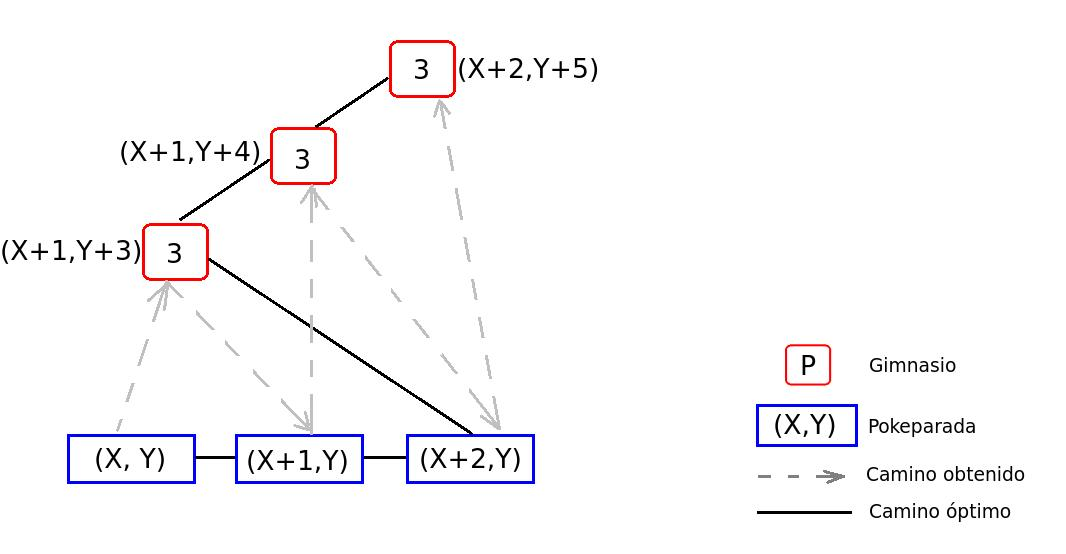
\includegraphics[scale=0.60]{./EJ2/nooptima.jpeg}
\\{\textit{La soluci\'on obtenida no es la \'optima}}
  \end{center}
  \vspace*{0.3cm}
  
La soluci\'on obtenida que dista de la \'optima puede ser tan mala como la cantidad de veces que se tenga que ir a una pokeparada, ganar gimnasio y luego ir a otra pokeparada a recuperarse por m\'as que esta \'ultima se encuentre mucho m\'as cerca de la pokeparada inicial que el gimnasio.

(ACA TENDRIA QUE HACER DOS DIBUJOS MAS NO OPTIMOS, EL QUE HICE ES EL PEOR DE LOS NO OPTIMOS, TENDRIA Q HACER UNO Q DISTE SOLO EN UN CAMINO Y OTRO Q DISTE UN POCO MAS)